\documentclass[aspectratio=169]{beamer}

\usetheme{Boadilla}
\usefonttheme{professionalfonts}
\setbeamertemplate{navigation symbols}{}
\setbeamertemplate{itemize items}[circle]
\setbeamertemplate{enumerate items}[default]
\setbeamertemplate{headline}{}

\usepackage[utf8]{inputenc}
\usepackage[T1]{fontenc}
\usepackage{lmodern}
\usepackage{amsmath}
\usepackage{booktabs}
\usepackage{tabularx}
\usepackage{array}
\usepackage{hyperref}
\usepackage[strings]{underscore}
\usepackage{listings}
\usepackage{tikz}
\usetikzlibrary{arrows.meta,positioning,fit,calc,shapes.geometric}
\usepackage{xcolor}

\definecolor{courseblue}{HTML}{12355B}
\definecolor{coursegold}{HTML}{C98A2E}
\definecolor{courseice}{HTML}{EEF3F8}
\definecolor{coursegreen}{HTML}{2F6B4F}
\definecolor{coursegray}{HTML}{4B5563}
\definecolor{codebg}{HTML}{F7F9FC}
\definecolor{codecomment}{HTML}{5E6C84}
\definecolor{codestring}{HTML}{0B6E4F}

\setbeamercolor{palette primary}{bg=courseblue,fg=white}
\setbeamercolor{palette secondary}{bg=coursegold,fg=white}
\setbeamercolor{palette tertiary}{bg=courseblue,fg=white}
\setbeamercolor{palette quaternary}{bg=coursegold,fg=white}
\setbeamercolor{structure}{fg=courseblue}
\setbeamercolor{frametitle}{bg=courseice,fg=courseblue}
\setbeamercolor{title}{fg=courseblue}
\setbeamercolor{block title}{bg=courseblue,fg=white}
\setbeamercolor{block body}{bg=courseice,fg=black}
\setbeamercolor{normal text}{fg=black,bg=white}
\setbeamercolor{alerted text}{fg=coursegold}

\setbeamerfont{footline}{size=\scriptsize}

\setbeamertemplate{footline}{
  \leavevmode
  \hbox{
    \begin{beamercolorbox}[wd=.33\paperwidth,ht=2.8ex,dp=1.2ex,leftskip=0.8em]{palette primary}%
      University of Trieste
    \end{beamercolorbox}%
    \begin{beamercolorbox}[wd=.49\paperwidth,ht=2.8ex,dp=1.2ex,center]{palette tertiary}%
      \coursename{} \textbar{} \coursecode
    \end{beamercolorbox}%
    \begin{beamercolorbox}[wd=.18\paperwidth,ht=2.8ex,dp=1.2ex,rightskip=0.8em plus1fil]{palette secondary}%
      \insertframenumber{} / \inserttotalframenumber
    \end{beamercolorbox}%
  }
}

\hypersetup{
  colorlinks=true,
  linkcolor=courseblue,
  urlcolor=coursegreen
}

\lstdefinestyle{coursepython}{
  language=Python,
  basicstyle=\ttfamily\footnotesize,
  keywordstyle=\color{courseblue}\bfseries,
  commentstyle=\color{codecomment}\itshape,
  stringstyle=\color{codestring},
  showstringspaces=false,
  columns=fullflexible,
  keepspaces=true,
  frame=single,
  framerule=0.6pt,
  rulecolor=\color{courseblue},
  backgroundcolor=\color{codebg},
  xleftmargin=0.4em,
  xrightmargin=0.4em,
  aboveskip=0.4em,
  belowskip=0.2em
}

\newcommand{\coursename}{Data-driven Systems Engineering}
\newcommand{\coursecode}{440MI / 305SM}
\newcommand{\coursefooter}{}

\newcommand{\learninggoals}[1]{
  \begin{block}{Learning goals}
  #1
  \end{block}
}

\newcommand{\repoactivity}[1]{
  \begin{block}{Repo activity}
  #1
  \end{block}
}

\newcommand{\readinglist}[1]{
  \begin{block}{Papers and materials}
  {\footnotesize #1}
  \end{block}
}

\newcommand{\coursecontextframe}[5]{
  \begin{frame}{Course Map and Running Cases}
  \centering
  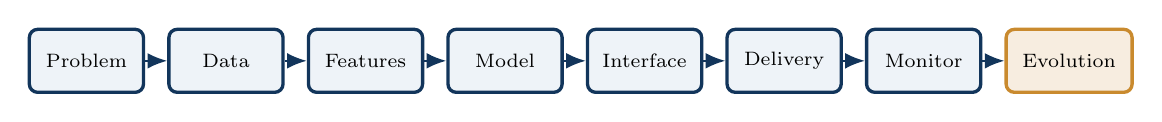
\begin{tikzpicture}[node distance=0.28cm]
  \node[flowbox, minimum width=1.45cm, minimum height=0.8cm] (problem) {\scriptsize Problem};
  \node[flowbox, minimum width=1.45cm, minimum height=0.8cm, right=of problem] (data) {\scriptsize Data};
  \node[flowbox, minimum width=1.45cm, minimum height=0.8cm, right=of data] (features) {\scriptsize Features};
  \node[flowbox, minimum width=1.45cm, minimum height=0.8cm, right=of features] (model) {\scriptsize Model};
  \node[flowbox, minimum width=1.45cm, minimum height=0.8cm, right=of model] (interface) {\scriptsize Interface};
  \node[flowbox, minimum width=1.45cm, minimum height=0.8cm, right=of interface] (delivery) {\scriptsize Delivery};
  \node[flowbox, minimum width=1.45cm, minimum height=0.8cm, right=of delivery] (monitor) {\scriptsize Monitor};
  \node[accentbox, minimum width=1.6cm, minimum height=0.8cm, right=of monitor] (evolution) {\scriptsize Evolution};
  \foreach \a/\b in {problem/data,data/features,features/model,model/interface,interface/delivery,delivery/monitor,monitor/evolution} {
    \draw[arrow] (\a) -- (\b);
  }
  \end{tikzpicture}

  \vspace{0.5em}
  \begin{block}{Today in the course}
  \textbf{Focus:} #1

  \textbf{Bridge:} #2
  \end{block}

  \begin{columns}[T]
  \column{0.48\textwidth}
  \begin{block}{Fraud case}
  {\footnotesize #3}
  \end{block}
  \column{0.48\textwidth}
  \begin{block}{Pasteurization case}
  {\footnotesize #4}
  \end{block}
  \end{columns}

  \vspace{0.3em}
  {\footnotesize \textbf{Course thread:} #5}
  \coursefooter
  \end{frame}
}

\newcommand{\classclosingframe}[4]{
  \begin{frame}{From This Class to the Next}
  \begin{block}{What stays with us}
  #1
  \end{block}

  \begin{columns}[T]
  \column{0.48\textwidth}
  \begin{block}{Project use}
  {\footnotesize #2}
  \end{block}
  \column{0.48\textwidth}
  \begin{block}{Next connection}
  {\footnotesize #3}
  \end{block}
  \end{columns}

  \vspace{0.3em}
  {\footnotesize \textbf{Course thread:} #4}
  \coursefooter
  \end{frame}
}

\tikzset{
  flowbox/.style={
    rounded corners=3pt,
    draw=courseblue,
    fill=courseice,
    very thick,
    minimum width=2.2cm,
    minimum height=0.9cm,
    align=center,
    font=\small
  },
  accentbox/.style={
    rounded corners=3pt,
    draw=coursegold,
    fill=coursegold!15,
    very thick,
    minimum width=2.2cm,
    minimum height=0.9cm,
    align=center,
    font=\small
  },
  arrow/.style={
    -{Latex[length=2.5mm,width=2mm]},
    thick,
    draw=courseblue
  }
}


\title{Class 3: Basic Python Programming}
\author{\coursename}
\date{}

\begin{document}

\frame{\titlepage \coursefooter}

\begin{frame}{Agenda}
\begin{itemize}
\item Variables and Python's dynamic typing.
\item Numbers, strings, and booleans.
\item Lists as Python's basic container type.
\item Modules, packages, and libraries: what the words actually mean.
\item The Python Standard Library and built-in functions.
\item Importing and using an external library.
\end{itemize}
\coursefooter
\end{frame}

\begin{frame}{Learning goals}
\learninggoals{
\begin{itemize}
\item Write and reason about variable assignment in a dynamically typed language.
\item Distinguish int, float, complex, string, and boolean values.
\item Build and modify a list using built-in methods.
\item Explain the difference between a module, a package, and a library.
\item Import a library and call a function from it with the correct syntax.
\end{itemize}
}
\coursefooter
\end{frame}

\coursecontextframe
{The smallest building blocks of Python: variables, types, and lists.}
{Every later notebook, script, and dashboard in this course is built from exactly these pieces, repeated at scale.}
{The fraud dashboard stores a transaction amount in a variable, a list of behavioral features in a list, and a model accuracy in a float --- three lines of code, three of today's topics.}
{The pasteurization simulator stores sensor readings the same way: plain variables and lists before anything is called a ``feature'' or a ``time series.''}
{Systems look complicated from the outside, but the vocabulary underneath is always variables, types, and containers.}

\begin{frame}[fragile]{Variables and dynamic typing}
\begin{lstlisting}[style=coursepython]
MODEL_ACCURACY = 0.9422
transaction_amount = 120.0
page_title = "Credit Card Fraud Detection"
\end{lstlisting}
\begin{itemize}
\item Variables are created with the assignment operator \texttt{=}; there is no separate type declaration.
\item Python is \textbf{dynamically typed}: a variable's type is decided by the value assigned to it, and can change later.
\item These three lines come straight from `streamlit/pages/App_Credit_Card.py`.
\end{itemize}
\coursefooter
\end{frame}

\begin{frame}{Rules for naming a variable}
\begin{itemize}
\item Must start with a letter or an underscore, never with a digit.
\item May contain only letters, digits, and underscores afterwards.
\item Names are case-sensitive: \texttt{amount} and \texttt{Amount} are different variables.
\item Conventionally lowercase with underscores for ordinary variables, uppercase for constants (as in \texttt{MODEL\_ACCURACY} above).
\end{itemize}
\coursefooter
\end{frame}

\begin{frame}{Arithmetic operators}
\begin{tabularx}{\textwidth}{>{\bfseries}l X}
Operator & Meaning \\
\toprule
\texttt{+} & Addition \\
\texttt{-} & Subtraction \\
\texttt{*} & Multiplication \\
\texttt{/} & Division (always returns a float) \\
\texttt{**} & Power \\
\texttt{//} & Integer (floor) division \\
\bottomrule
\end{tabularx}
\coursefooter
\end{frame}

\begin{frame}{Numeric types}
\begin{itemize}
\item \textbf{int}: whole numbers, such as a count of transactions or students in a group.
\item \textbf{float}: decimal numbers, such as \texttt{MODEL\_ACCURACY = 0.9422} or a sensor reading.
\item \textbf{complex}: numbers with a real and imaginary part; rarely needed in this course, but part of the standard set.
\item Python decides which of these a literal is the moment it is written: \texttt{10} is an int, \texttt{10.0} is a float.
\end{itemize}
\coursefooter
\end{frame}

\begin{frame}[fragile]{Strings}
\begin{lstlisting}[style=coursepython]
st.title("Credit Card Fraud Detection System")
message = "Adjust the sliders to simulate a transaction."
label = "Feature V" + str(1)
\end{lstlisting}
\begin{itemize}
\item Strings can be written with single or double quotation marks; this course mostly uses double quotes.
\item Strings behave like arrays of characters and can be indexed, e.g.\ \texttt{label[0]}.
\item Concatenation uses \texttt{+}, but only between strings --- numbers must be converted with \texttt{str()} first.
\end{itemize}
\coursefooter
\end{frame}

\begin{frame}{Booleans}
\begin{itemize}
\item Python's boolean type has exactly two values: \texttt{True} and \texttt{False}.
\item Comparisons such as \texttt{prediction == 1} or \texttt{probability > 0.5} evaluate to a boolean.
\item Boolean logic uses English keywords rather than symbols: \texttt{and}, \texttt{or}, \texttt{not}.
\item Booleans decide almost every branch of code we will write from next class onward.
\end{itemize}
\coursefooter
\end{frame}

\begin{frame}[fragile]{Lists}
\begin{lstlisting}[style=coursepython]
user_inputs = []
user_inputs.append(0.0)

input_data = [transaction_amount] + user_inputs
print(len(input_data))
\end{lstlisting}
\begin{itemize}
\item A list is Python's ordered, resizable container; elements do not need to share a type.
\item \texttt{.append()} is a built-in list method; \texttt{+} between two lists concatenates them.
\item `App\_Credit\_Card.py` builds exactly this kind of list to collect the 28 behavioral features of a transaction.
\end{itemize}
\coursefooter
\end{frame}

\begin{frame}{Modules, packages, and libraries}
\begin{itemize}
\item A \textbf{module} is one file of Python code: functions, classes, and variables collected together.
\item A \textbf{package} is a directory of modules, marked so Python can import from it.
\item A \textbf{library} is a collection of modules and packages meant to be reused across projects.
\item The Python Standard Library ships with the interpreter: file I/O, basic mathematics, and much more, with no installation needed.
\end{itemize}
\coursefooter
\end{frame}

\begin{frame}[fragile]{A first look at the Standard Library}
\begin{lstlisting}[style=coursepython]
import math

math.sqrt(16)      # 4.0
math.log10(1000)   # 3.0
math.pi            # 3.14159...
\end{lstlisting}
\begin{itemize}
\item The \texttt{math} module ships with every Python install: trigonometric, logarithmic, and constant values.
\item \texttt{statistics}, another Standard Library module, adds \texttt{mean()} and \texttt{stdev()} without installing anything.
\end{itemize}
\coursefooter
\end{frame}

\begin{frame}{A handful of built-in functions}
\begin{tabularx}{\textwidth}{>{\bfseries}l X}
Function & What it does \\
\toprule
\texttt{len()} & Number of elements in a list, string, or other container. \\
\texttt{type()} & The type of a value, useful while debugging dynamic typing. \\
\texttt{print()} & Writes to standard output; the most-used function in this course. \\
\texttt{sum()} / \texttt{sorted()} & Aggregate or order the elements of a list. \\
\texttt{range()} & Generates a sequence of integers, mostly seen together with loops. \\
\bottomrule
\end{tabularx}
\coursefooter
\end{frame}

\begin{frame}[fragile]{Importing an external library}
\begin{lstlisting}[style=coursepython]
import streamlit as st
import numpy as np
import pandas as pd
\end{lstlisting}
\begin{itemize}
\item \texttt{import x as y} imports the whole library under a short alias --- these three aliases are used everywhere in this repository.
\item Standard Library modules (\texttt{math}, \texttt{statistics}) never need installation; external libraries (\texttt{streamlit}, \texttt{numpy}, \texttt{pandas}) do, which is exactly what `requirements.txt` is for.
\end{itemize}
\coursefooter
\end{frame}

\begin{frame}{How the repo already uses today's building blocks}
\repoactivity{
\begin{itemize}
\item `streamlit/pages/App_Credit_Card.py` opens with plain variables (\texttt{MODEL\_ACCURACY}), a list (\texttt{user\_inputs}), and library imports before anything ML-specific happens.
\item `streamlit/modeling.py` stores a dataset URL in a string variable and a target column name in another --- the exact pattern from today's slides.
\item Skim either file and count how many lines are only variables, types, or imports before the first model-specific call.
\end{itemize}
}
\coursefooter
\end{frame}

\begin{frame}{Discussion prompt}
\begin{block}{Question}
If a variable's type can change at any time in Python, what could go wrong in a long script, and how would you protect against it?
\end{block}
\begin{itemize}
\item Surfaces the trade-off behind dynamic typing before students hit a confusing type error later in the course.
\item Motivates disciplined naming and, eventually, type hints.
\end{itemize}
\coursefooter
\end{frame}

\begin{frame}{Papers and materials}
\readinglist{
\href{https://jupyter.org/install}{Jupyter install guide};\
\href{https://pandas.pydata.org/docs/}{pandas documentation};\
Chip Huyen, \textit{Designing Machine Learning Systems};\
Noah Gift and Alfredo Deza, \textit{Practical MLOps}.
}
\coursefooter
\end{frame}

\classclosingframe
{\begin{itemize}
\item Variables, numeric and string types, booleans, and lists are the vocabulary every later script reuses.
\item Modules, packages, and libraries describe how Python code is organized and shared, not just where files live.
\item Reading real repository files is already possible once these basics are solid.
\end{itemize}}
{Before writing project code, make sure you can read a file like `App_Credit_Card.py` line by line and name what each line does.}
{Class 4 moves into control flow --- conditionals, loops, and dictionaries --- so these values can start driving decisions rather than sitting still.}
{Today's static values become tomorrow's dynamic behavior.}

\end{document}
